\chapter{State of the Art}
\label{chp:sota}
In this chapter we examine work that has been done in using deep learning for recommender systems. In particular, we are interested in the use of RNNs and the session-based recommender system setting.

\section{Other approaches}
Here we briefly mention some of the most used or successful non-RNN approaches to recommender systems.

\subsection{The item-to-item approach}
In recommender systems where a user profile is available, Matrix factorization and neighborhood models have been among the most popular approaches. Due to the missing user information on the session-based scenario, these methods do not work well there. In session-based recommendations, a popular approach is item-to-item recommendation. The item-to-item method precomputes a similarity matrix for the items. Items who are similar, based on the available session data, get high scores, and recommendation is done simply by recommending similar items. Similarity is calculated by looking at which items are often clicked in the same sessions. This method is simple and effective, and has been widely used \cite{DBLP:journals/corr/HidasiKBT15}. However, it only takes into account the last click.

\subsection{Markov models}
Markov models are able to representing time dependencies. Hidden Markov models model an observed sequence as probabilistic dependent on a sequence of unobserved states \cite{DBLP:journals/corr/Lipton15}. The problem is that as the time window grows, the state space grows exponentially. This makes Markov models infeasible on longer sequences. RNNs do not have this problem, because the number of states that can be represented grows exponentially with the number of nodes in a layer. In addition, the complexity of inference and training grows at most quadratically \cite{DBLP:journals/corr/Lipton15}.

\subsection{Deep learning}
Restricted Boltzmann Machines (RBM) have successfully been used for collaborative filtering \cite{Salakhutdinov:2007:RBM:1273496.1273596} \cite{DBLP:journals/corr/HidasiKBT15}, and has been shown to be one of the best performing models for that approach. The RBM model performs recommendations based on modeling user-item interaction.

Deep models have also been used to extract content features, and then combined with a collaborative filtering model to enhance the results \cite{DBLP:journals/corr/WangWY14} \cite{Oord:2013:DCM:2999792.2999907} \cite{DBLP:journals/corr/HidasiKBT15}.

In 2015, Wan et al. \cite{conf/recsys/WanLWGXC15} experimented with a three layered neural network for next basket recommendation. A basket here refers to the shopping basket on an e-commerce site. So the setting is a e-commerce site where users have done some purchases, where each purchase consists of a basket with one or more items. In this scenario the recommender system has access to the users history, so it is not a session-based problem. Wan et al. argues that recommendations should be based on the full user history, not only the last purchases. To illustrate, a user might purchase a computer, then he might purchase groceries in his next basket, and then he wants to buy some accessories to his computer. They feed the network with the user history by creating vectors that represent the average of each basket, and creating an embedded concatenation of these vectors. Their network outperforms the baselines they compare it to.

\begin{figure}[htp]
	\centering
	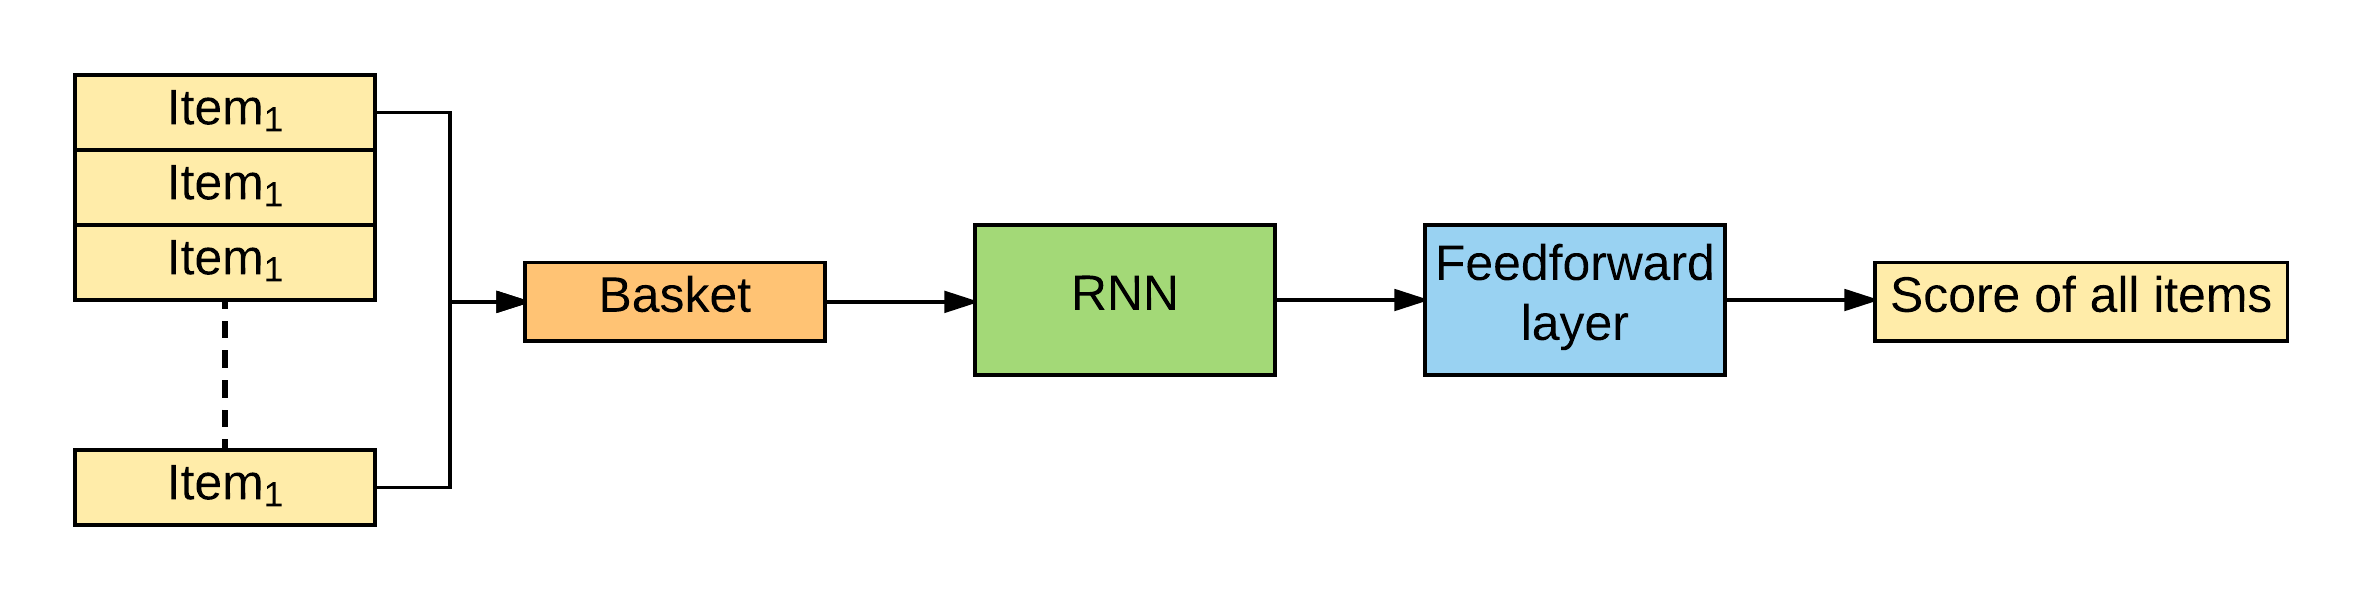
\includegraphics[width=1.0\textwidth]{fig/rnn-next-basket.png}
	\caption{General architecture of the RNN from ''A dynamic recurrent model for next basket recommendation'' by Yu et al. \cite{Yu:2016:DRM:2911451.2914683}}
	\label{fig:rnn-next-basket}
\end{figure}

A paper by Yu et al. from 2016 \cite{Yu:2016:DRM:2911451.2914683} suggests using a RNN to perform next basket recommendation. Their network architecture is illustrated in Figure \ref{fig:rnn-next-basket}. They represent each user basket by pooling together the item vectors in the basket. The basket representation is sent through a simple RNN and outputs a vector with a score for each item. Their model performs better than the baselines over two datasets. This is not a session-based recommender system, but in the next section we look at a paper that applies a similar model as a session-based recommender.


\section{Session-based recommendations with recurrent neural networks}
\label{sec:hidasi-sess-based-rnn}
Hidasi et al. published the paper ''Session-based Recommendations with Recurrent Neural Networks'' in 2016 \cite{DBLP:journals/corr/HidasiKBT15}. This paper proposes to use a RNN for session-based recommendations, and shows that a basic RNN can achieve remarkable results. They also deal with sparsity issues, and introduce a new ranking loss function for training the network. Their general network architecture is shown in Figure \ref{fig:gru4rec-network}. The proposed network is pretty straightforward, this is also the first RNN architecture discussed in this paper, therefore we will go through the layers in detail.

\begin{figure}[htp]
	\centering
	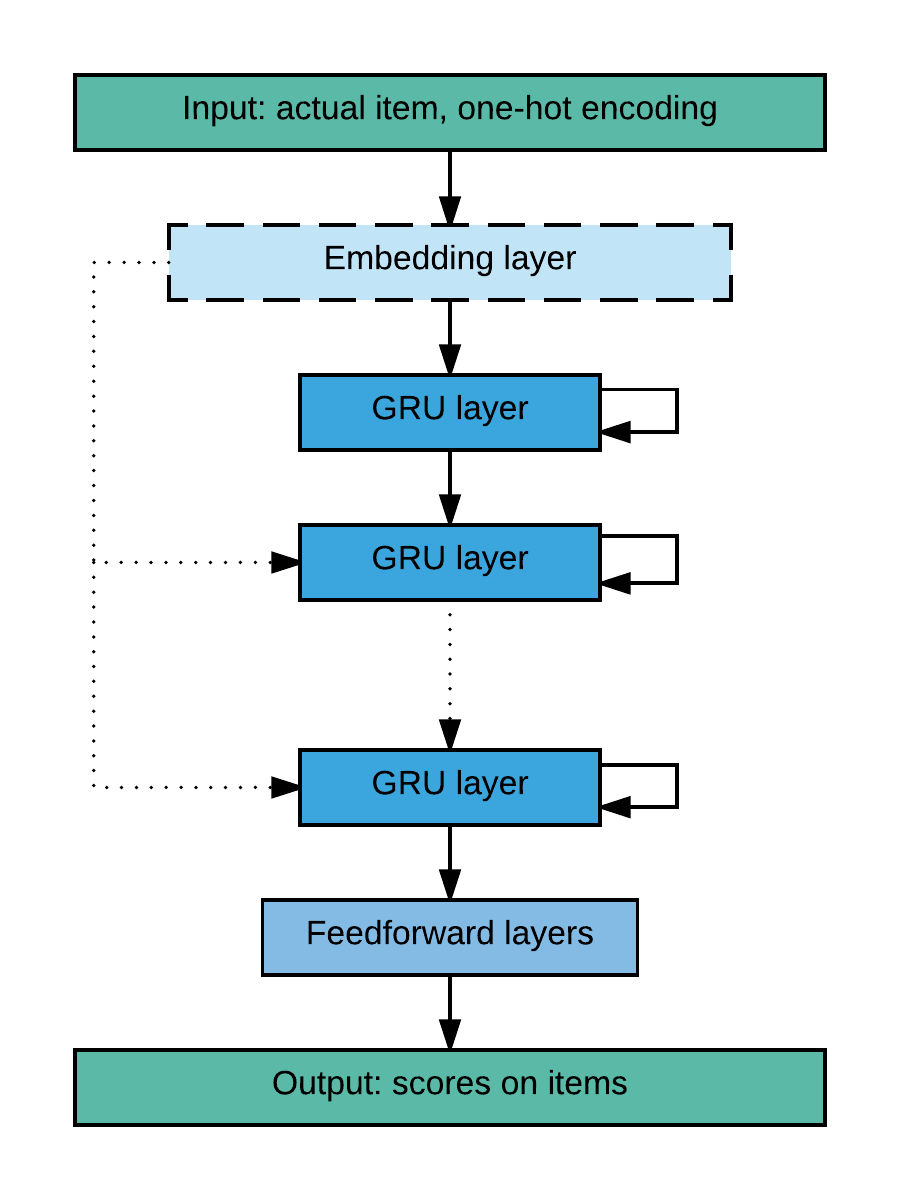
\includegraphics[width=0.5\textwidth]{fig/gru4rec-network.png}
	\caption{General architecture of the RNN from ''Session-based recommendations with recurrent neural networks''. \cite{DBLP:journals/corr/HidasiKBT15}}
	\label{fig:gru4rec-network}
\end{figure}

They experimented with two different datasets. Both datasets contains sequences of user clicks with timestamps. One dataset has clicks on items from an e-commerce site from the RecSys Challenge 2015 \cite{dataset:recsys15}, while the other contains clicks on videos from a YouTube-like platform. Various modifications of the network in Figure \ref{fig:gru4rec-network} were tested. We discuss these as we explain the architecture, layer by layer.

\subsection{Input layer}
Two different ways of encoding the input were compared. The first encoding was a pure one-hot encoding. The second was a weighted sum of the first representations, where earlier events are discounted, and the entire vector was normalized before fed into the network. Adding information about all earlier events could possibly help the to reinforce the memory effect. However, in this case the RNN performed better with the pure one-hot encoding. 

\subsection{Embedding layer}
In the paper, the authors mention that they experimented with using an embedding layer between the input- and the RNN layer. Their results were always better without the embedding layer. However, if the performance loss is small, an embedding layer can still be useful to speed up calculations, as mentioned in \ref{sec:embeddings}. In the recommender system setting, the number of possible items can be very large, also the system need to be responsive, so potential speed optimizations should be considered.

\subsection{GRU layers}
GRU units outputs a hidden state and an output which is the prediction for the time step. The hidden state from each layers is inputted back into the same layer for each time step, but it is also fully possible to output the hidden state to the next layer, instead of or in addition to the prediction output. The authors experimented with using multiple GRU layers, where they used the hidden state as output to the next layer, except for the last GRU layer which outputted the prediction output. Best performance was achieved with a single GRU layer. It is not clear why additional layers did not improve the result, but as the authors mention, it might be because the sessions have short lifespans. If the sessions spanned over weeks, then additional layers could catch user features at different time scales. I.e. one layer could learn the more static features of the user, features which does not change over the whole session. While another layer could learn the more temporal user features, features that were only present for the past hour for example. It was also found that, when using multiple GRU layers, feeding the input, the one-hot- or the embedded vector, into the deeper GRU layers resulted in better performance.

\subsection{Feedforward layers}
In the paper, they found that using a single feedforward layer gave the best results. The feedforward layer maps a smaller vector to the same size as the input layer, where each item corresponds to one index again. By having a feedforward layer between the GRU layer and the output, the GRU layer can be much smaller. Since a GRU layer is more complex than a feedforward layer, it is also slower in terms of computations. In recommender systems, the number of items can span from thousands to millions. Therefore, keeping the GRU layer small can be necessary to achieve a feasible runtime.

\subsection{Training}
The e-commerce dataset has about 40 000 items, while the video dataset has about 330 000 videos. Therefore, the paper samples the output, and only calculates scores for some of the outputs. The network outputs a score for each item, since the output vector contains one value in each index. The correct output is one where the desired item, the next one in the session, has a higher score than the others. There are at least two reasons why the other items in each time step were not clicked. One possibility is that the user did not see the item. Another possibility is that the user saw the item, but chose to not click it, because it was not interesting to the user. For popular items, the second reason is more likely, and it is important that the network learns to give these items a low score. In the paper, this is solved by using the items from the other examples in the current mini-batch as negative examples, and of course, the next click is the positive example. By using clicks from the other examples in the mini-batch, computations for sampling is saved, in addition, these clicks are sampled by proportion to how popular they are, because popularity is decided by number of clicks.

In the paper, Bayesian Personalized Ranking \cite{Rendle:2009:BBP:1795114.1795167}, TOP1 (devised by the authors \cite{DBLP:journals/corr/HidasiKBT15}), and cross-entropy are used to calculate the loss. With 100 units in the GRU layer, cross-entropy performed best. With 1000 units, TOP1 performed best overall, but was beaten by BPR on one metric. TOP1 performed better with 1000 units, than cross-entropy did with 100.

\subsection{Evaluation metrics}
\label{sec:evaluation-metrics}
The paper suggests two performance metrics suited for recommender systems.

\subsubsection{Recall@N}
In cases where the recommender system can recommend a set of N items, and the full set is visible to the user, it is important that good recommendations are in the set, but the ordering does not matter. The Recall@N measure is then how often the correct next click is present in the top N recommendations by the recommender system. The top N recommendations are the N items with the highest score given by the system.

\subsubsection{MRR@N}
When the user needs to do some form of scrolling to see all recommendations, the order of the recommendations becomes important. The best recommendations should be the first visible to the user. Mean reciprocal rank (MRR) covers this case. MRR@N measures the average of the reciprocal rank of the correct click in the systems ordered N recommendations. If the system recommends 20 items, then it gets a score of 0 if the correct prediction is not in the list of recommendations. If the correct prediction is in the list, the system gets a score of $\frac{1}{i}$, where $i$ is the rank in the list. So if the correct item is first in the list, the score is $\frac{1}{1} = 1$, and if it is number five in the list, the score is $\frac{1}{5} = 0.2$. The MRR@N is the average of these scores over all the test examples.

\subsection{Results and Conclusion}
The RNN in the paper was compared to several baselines. The best performing baseline was the item-KNN. Item-KNN recommends items based on similarity, where the similarity is calculated based on items co-occurrences in sessions. This similarity is calculated with the cosine similarity between the vector of the sessions where both items occur. Specifically it is ''the number of co-occurrences of two items in sessions, divided by the square root of the product of the number of sessions in which the individual items occured'' \cite{DBLP:journals/corr/HidasiKBT15}.

This simple item-to-item method is usually a strong baseline, and often used in practice. The paper's proposed RNN significantly outperforms the item-KNN baseline with about 15 - 30 \% higher accuracy scores on the two evaluation metrics. The paper by Hidasi et al. has given us a solid RNN, with a relatively simple architecture. It performs well even though it only looks at the sequences of item clicks. No additional information about the items are fed into the network. The next papers we discuss looks at methods that can be used to further improve results.



\section{Improving RNNs for session-based recommendations}
Tan et al. \cite{DBLP:journals/corr/TanXL16} looks at various ways of improving the model proposed Hidasi et al. in \cite{DBLP:journals/corr/HidasiKBT15}. They experiment with techniques that have worked well when neural networks have been applied to other problems, to see if those techniques can improve performance of a RNN session-based recommender as well. The same evaluation metrics, Recall@20 and MRR@20, were used, and they experimented on the same dataset \cite{dataset:recsys15}. They suggest four techniques, and train one model with each technique. The four models are then compared with each other and a baseline which is the model proposed by Hidasi et al. in \cite{DBLP:journals/corr/HidasiKBT15}.

\subsection{Data augmentation}
Based on \cite{DBLP:journals/corr/BrebissonSAVB15}, they generate multiple sequences from each sequence in the original dataset. For a sequence \lbrack $x_1$, $x_2$, ..., $x_n$\rbrack, they create sequences \lbrack $x_1$, $x_2$\rbrack, \lbrack $x_1$, $x_2$, $x_3$\rbrack, ..., \lbrack $x_1$, $x_2$, ..., $x_{n-1}$\rbrack, in addition to the original sequence. The last click in each sequence is used as the target click.

Another form of data augmentation they suggest is dropout performed on the click in the training sequences. This is based on results from \cite{rnn-dropout}. By randomly dropping clicks in the training sequences, the model could become less sensitive ti noise clicks, which makes the model less prone to overfitting on noise. Both methods are illustrated in Figure \ref{fig:sequence-augmentation}. The models described in this section will be referred to as M1.

\begin{figure}[htp]
	\centering
	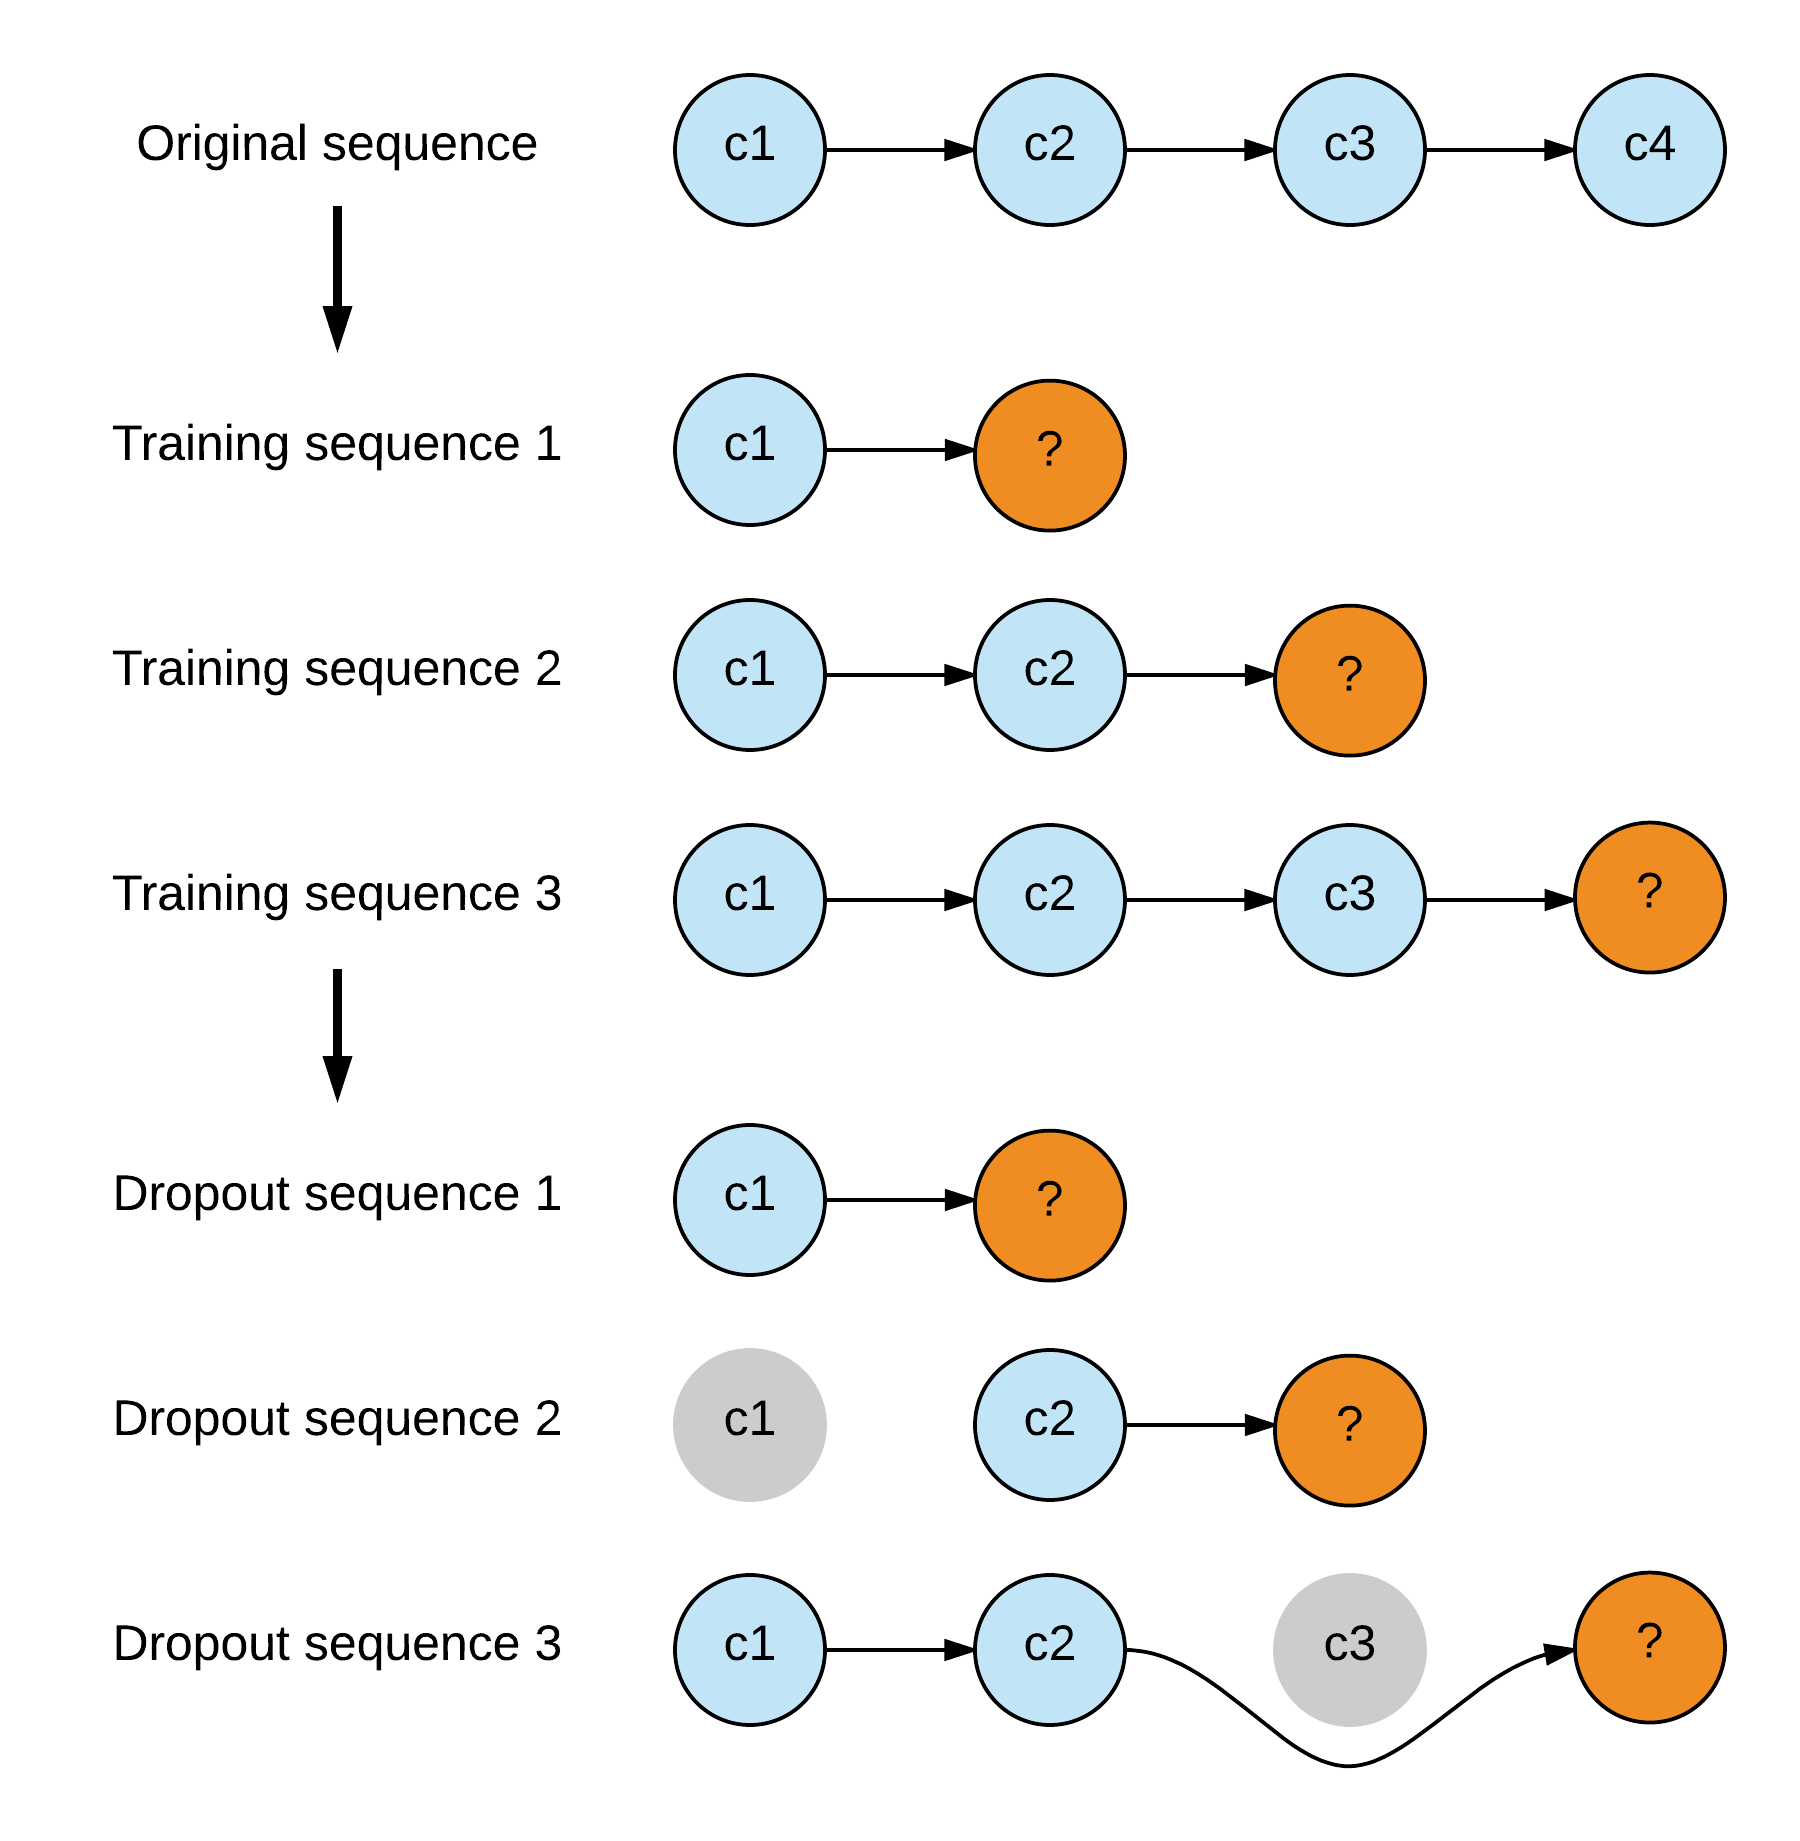
\includegraphics[width=0.7\textwidth]{fig/sequence-augmentation.png}
	\caption{Data augmentation for training sequences as suggested in \cite{DBLP:journals/corr/TanXL16}. Multiple training sequences are generated from a original sequence. Random dropout is applied to the clicks in the sequences.}
	\label{fig:sequence-augmentation}
\end{figure}

\subsection{Pre-training to adapt to temporal changes}
In the session-based setting, the items available for recommendation changes over time. One of the consequences is that users interest change over time, as newer items are often more exciting than old ones. These changes will be reflected in the training sequences, where the most recent examples more correctly reflects users interests. Naturally, the recommender system should be in sync with the users current preferences. One obvious solution is to discard examples from the dataset that are older than a certain threshold. However, this means a lot of data is lost. It would be better if this data could be utilized. Tan et al. suggests that a good solution is to apply pre-training. First the model is trained on the whole dataset, then it is fine-tuned on only the most recent examples. This results in a model that makes use of the full dataset, but which is focused more on the recent tendencies. This idea is based on the fine-tuning often used on image-based networks \cite{DBLP:journals/corr/ChatfieldSVZ14}. The models described in this section will be referred to as M2.

\subsection{Privileged information}
When training on a subsequence of a session, there is still the remaining part of the sequence, which contains information about the session. Tan et al. proposes to use this information as well when training. Look at Figure \ref{fig:rnn-teacher-student} for an illustration.

\begin{figure}[htp]
	\centering
	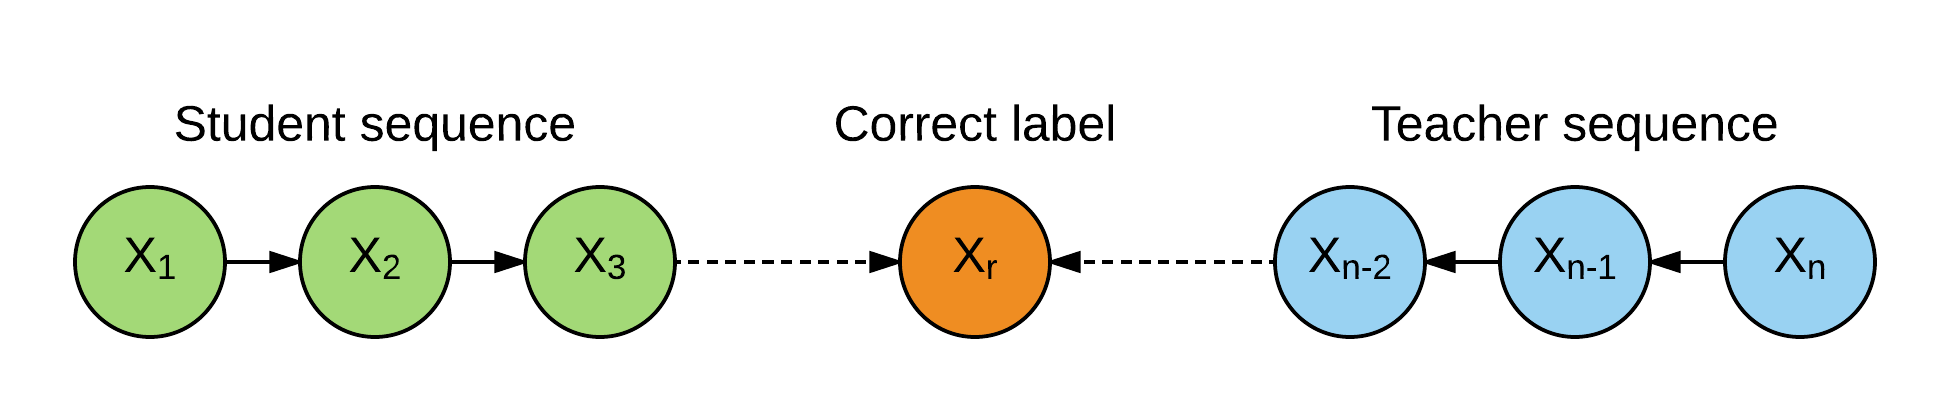
\includegraphics[width=1.0\textwidth]{fig/rnn-teacher-student.png}
	\caption{Data augmentation with teacher labels as suggested in \cite{DBLP:journals/corr/TanXL16}. The student model is trained to predict a tradeoff between the real label and the label predicted by the teacher model. The label produced by the teacher model is the teacher model's prediction of the correct label but on the remainder of the sequence in reverse.}
	\label{fig:rnn-teacher-student}
\end{figure}

For some sequence \lbrack $x_1$, $x_2$, ..., $x_r$, ..., $x_{n-2}$, $x_{n-1}$, $x_n$\rbrack, where $x_r$ is the label, the model is being trained to predict $x_r$ based on \lbrack $x_1$, $x_2$, ..., $x_{r-1}$\rbrack. This is normal training as we have already looked at. The addition is that the label that the model is trained to predict is substituted with a tradeoff between the correct label and a label produced by a teacher model. The label produced by the teacher model, is the teacher model's prediction of the correct label, $x_r$ based on the reverse of the remaining sequence, which is \lbrack $x_n$, $x_{n-1}$, ..., $x_{r+1}$\rbrack. This approach can be useful when the available training data is small, such as for new website \cite{DBLP:journals/corr/TanXL16}. The models described in this section will be referred to as M3.

\subsection{Output embeddings}
Since the number of possible items to recommend can be huge, which means that outputting a vector of size equal to the number of items requires a lot of calculations, which means that the model can become less responsive (slow to calculate an output). To deal with this \cite{DBLP:journals/corr/TanXL16} suggests to output an item embedding instead of a full item vector. Since the embedding is a smaller vector, this means less calculations and faster predictions. The top N recommendations are extracted from the output embedding by finding the items most similar embeddings in the embedding space, where similarity is calculated with cosine similarity. For this to work, the model needs to have good embeddings to train on. The authors suggests using the embeddings found with one of the other models for this. The models described in this section will be referred to as M4.

\subsection{Results and conclusion}
The RecSys Challange 2015 dataset was preprocessed and split into test and training sets in the same way done by Hidasi et al. in \cite{DBLP:journals/corr/HidasiKBT15}. To better evaluate their models, the authors sorted the training set by time and compared using the most recent fractions ($\frac{1}{256}$, $\frac{1}{64}$, $\frac{1}{4}$, $\frac{1}{1}$) of the training sequences. The same evaluation metrics were used. As baseline, the pest reported results from \cite{DBLP:journals/corr/HidasiKBT15} were used.

Except when only using the most recent fraction of the training data ($\frac{1}{256}$), all proposed models, M1-M4, performed better than the baseline. M4 generally performed worst of the four models. M2 performed best, especially on the most recent fractions. M2 was not trained on the whole training set, since that would be equivalent to recreating the baseline. M1 and M3 performed best when trained on $\frac{1}{4}$ and $\frac{1}{16}$ of the most recent training examples. At best, M2 achieved about 10 percentage points better on Recall@20 and about 8 percentage points better on MRR@20 than the baseline. However, it might have been a bit unfair to use the reported performance from \cite{DBLP:journals/corr/HidasiKBT15} as a baseline. Hidasi et al. did many optimizations to make their model run faster \cite{email:Hidasi}, and some of the tricks they used might have lowered the models performance (in terms of Recall@20 and MRR@20) in a tradeoff for faster runtime. The M2 model trained on the full training set would probably have been a more fair baseline to compare the models to. Based on the results for M2 on the fractions of the training set it was trained on, it seems reasonable to believe that M2 would have gotten a significant better score than the baseline when trained on the full training set.

Still the paper presents some nice ideas on how to improve a RNN session-based recommender. Dropping some of the oldest data can improve the results for any model. Also, the M4 model had about half the prediction time of the other models, which is useful in cases where one wants to do a tradeoff.


\section{Utilizing context information}
So far we have looked at models that performs predictions solely based on the items clicked, where the items are only represented by an id in the form of a one-hot vector. Clearly, additional information, both about the item and about the sessions, could help improve the predictions. Some possible additional information about the item is be the category of the item, an image, and a textual description of the item. Additional information about the session could be timestamps of the clicks, geolocation of the user, and weather. In this section we discuss a paper that examine if and how additional information can improve a RNN recommender.

We start in this section by looking at ''Context-aware sequential recommendation'' by Liu et al. \cite{DBLP:journals/corr/LiuWWL016}.

The paper suggests that modeling the time of a session and the transition time between events in the session both can give better performance. Modeling time, such as hour of the day and day of the week, can help the model capture tendencies that depend on when a session occur. As an example, think of a music streaming service. During working hours on the weekdays, users might listen more to calm music which helps them concentrating. On the evening in the weekend, there might be a rush in users listening to party music at parties. And music preferences might vary with the seasons of the year. The authors refer to this as input contexts.

Time between actions in a session might give indication about how relevant actions are to each other. Intuitively, actions that happens in short time intervals should be more relevant to each other, and visa versa. This could help the RNN decide when to what to forget and what to remember. The authors refer to this as transitional contexts.

Liu et al. proposes to define a finite number of input and transitional contexts and then give the recommender model one layer for each context. When an example is given to the model, it uses only the appropriate layers, and similarly training is done on the layers that were used for the example. More technically, the item input vector is multiplied with a input context matrix, and the hidden state vector is multiplied with a transition context matrix in each step in a sequence. It is these matrices that the authors suggest to generate for each possible context. The input contexts used in the paper are 24 hours of the day, seven days of the week, three ten-day periods in a month, and holiday or not. There can be an infinite amount of time intervals between two user actions, so the authors suggests to split the transitional contexts into bins. E.g. less than one hour, 1-2 hours, 2-3 hours, and more than three hours.

The authors does not explain how the different context matrices are trained on different data, but an approach that seems reasonable is the pre-training from \cite{DBLP:journals/corr/TanXL16}. A common matrix could be trained on the full dataset, independent of the different contexts, and this matrix could then be used as the initialization for the multiple context matrices. Instead of using multiple context matrices, the input context could be fed to the model as additional input. This would make the model simpler.

Two datasets were used in the paper. Taobao \cite{dataset:taobao} and Movielens-1M \cite{dataset:movielens}, which both have contextual information in the form of timestamps. The authors compared their context-aware model to several baseline. Simple baselines such as only recommending the most popular items, context-aware baselines, and sequential methods such as standard RNN were used. Also, to compare the effect of the two contexts, the authors created two models with only input or transition contexts.

The context-aware model performed significantly better than all the compared baselines, on both datasets. It also performed better than the two models restricted to only one context. Those two models performed similarly to each other. All three context models performed significantly better than the standard RNN which performed best among the baselines.

These results strongly supports the idea that recommender systems should consider available context information in their recommendations. Note that even though, the paper only experiments with contextual information in RNNs, it seems reasonable to believe that the benefit could be applied to other recommender systems as well. The benefits of utilizing input context should not be constricted to only sequence prediction either.


\section{Multi-rate learning}
In ''Multi-rate deep learning for temporal recommendation'' by Song et al. \cite{Song:2016:MDL:2911451.2914726}, they test how modeling both long- and short-term user preferences can improve a recommender system. The authors proposed model uses available user history, but the ideas should be transferable to the session-based setting.

The basic assumption of the paper is that user interests change over time. As an example, in \cite{Elkahky:2015:MDL:2736277.2741667}, it was shown that users who visited spligle.de, a popular German news portal, were likely to be interested in football related news. The reason was that the data was collected around the time of the football world cup of 2014 \cite{Song:2016:MDL:2911451.2914726}. Similarly, user interests may change over time, e.g. during summer and Christmas. The authors propose to use a model that combines static and temporal user features. The static features are learned by using the full training set, while the temporal features are learned by only training on the most recent examples. The question is then what the threshold for what is considered recent is. The results from \cite{DBLP:journals/corr/TanXL16} showed that using only very recent examples gave worse performance than with with a more relaxed threshold. At the same time, accepting too old examples means that the model will not be able to capture the current user interests. Song et al. proposes a multi-rate model, which use two separate RNNs of different temporal granularity to deal with this.  To deal with the large amount of parameters the two RNNs entail, they use pre-training.

Pre-training is done differently here than in \cite{DBLP:journals/corr/TanXL16}, which we discussed earlier. Song et al. pre-trains embeddings of the item features and the user static features. These embeddings are then used as input in the multi-rate model. Since the embeddings are smaller in dimensionality than original input vectors, the result is fewer parameters to train in the multi-rate model.

The proposed model that combined a RNN adopted to very recent user interests and a RNN adopted to more long term shifts, outperformed the compared baselines significantly. The results supports the idea that a session-based recommender system should focus on recent user behaviors, without discarding old behaviors. However, these results might be affected by the smaller amount of training examples available when only focusing on the most recent behavior.


\section{Modeling event information}
Often, there is more information about a session available than just the items clicked and timestamps. For an e-commerce site this information might include what type of action the user performed, such as viewing an item, adding it to the basket, removing it from the basket, or buying it. Websites often have a search field , which both get a lot uf user interaction as well as information through the search queries. In ''Modelling contextual information in session-aware recommender systems with neural netwrks'' \cite{Twardowski:2016:MCI:2959100.2959162}, Twardowski proposes a RNN model that makes use of this information for it's recommendations. The proposed model sends embedded event information through a RNN layer, the output is concatenated with an embedded item representation, before being sent through feed forward layers to produce a prediction. On a dataset with rich search contextual information, the proposed RNN model performs significantly best. While on a dataset with less events and data, the RNN model performed worse than a matrix factorization model that was also customized to utilize event information.


\section{Parallell RNN for feature-rich sessions}
In ''Parallell recurrent neural network architectures for feature-rich session-based recommendations'' \cite{Hidasi:2016:PRN:2959100.2959167} Hidasi et al. expands upon the work from \cite{DBLP:journals/corr/HidasiKBT15} and try to model richer representations of the clicked items in sessions. Since e-commerce sites often have both a picture and textual description of items, it is desirable to use this information to make better predictions. The authors suggests four different architectures that take both the item id, represented by a one-hot vector, and an image feature vector (or text feature vector) as input and computes scores on items. Also, they used two models that only had one of the vectors as input, to form baselines for comparison. The best performing architecture they proposed is illustrated in Figure \ref{fig:parallell-rnn}.

\begin{figure}[htp]
	\centering
	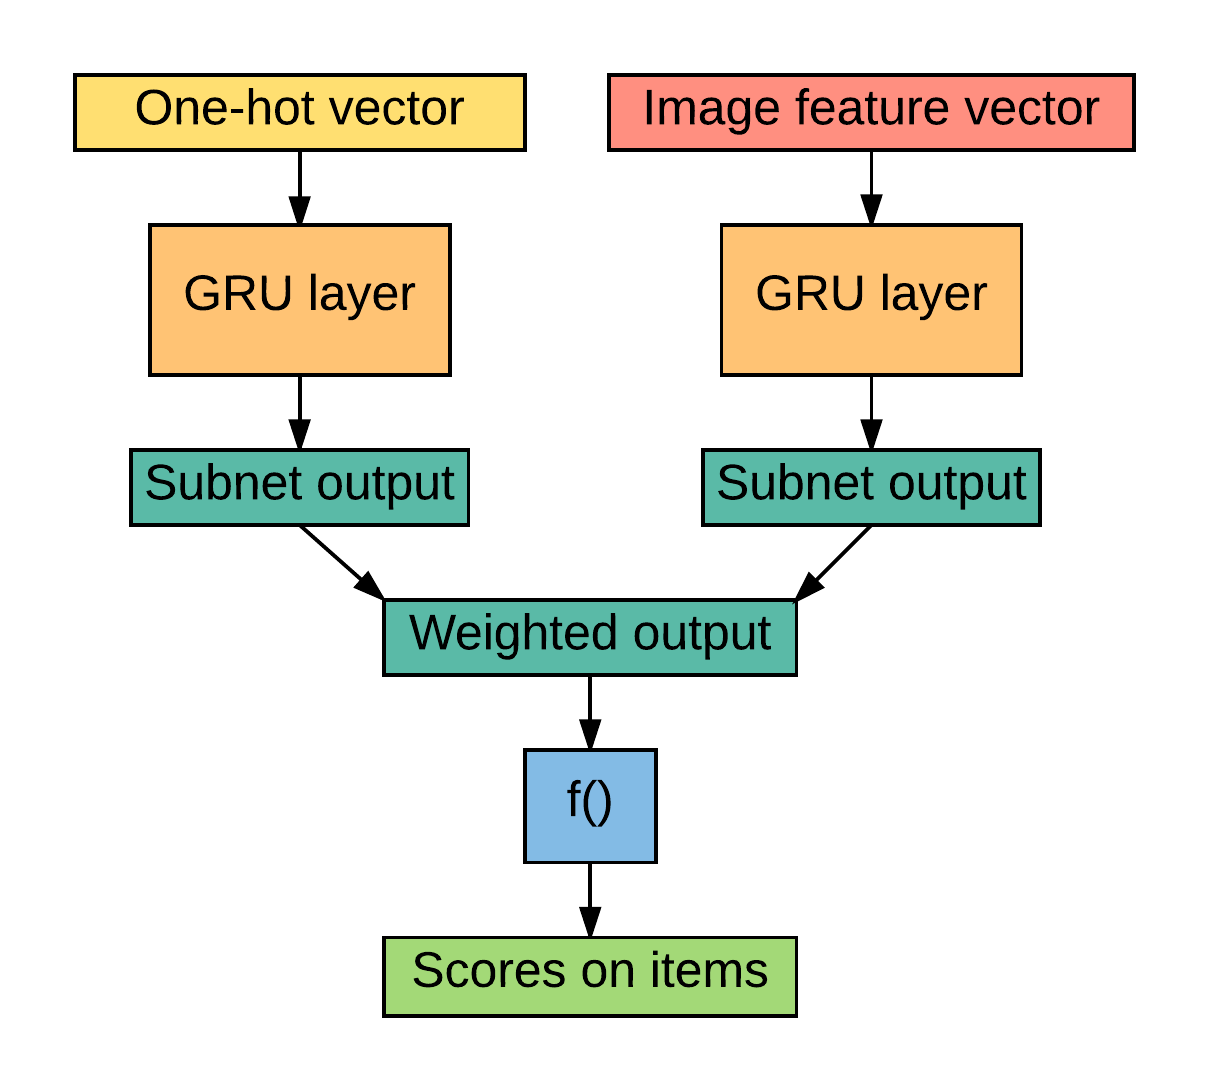
\includegraphics[width=0.7\textwidth]{fig/parallell-rnn.png}
	\caption{One of the proposed architectures from \cite{Hidasi:2016:PRN:2959100.2959167}. The image feature vector can be replaced with a text feature vector. f() is a nonlinearity applied to the output, in the paper they used tanh.}
	\label{fig:parallell-rnn}
\end{figure}

The two input vectors are fed into two separate GRU layers, and the outputs are combined by weighting each output. Lastly, the combined output is sent through an activation layer, giving scores for all possible items. The target label is the one-hot representation of the next event in the session. Two datasets were used, one with images of the items, and one with textual descriptions. The authors suggest different ways of training the models. Standard backpropagation can be suboptimal due to the parallelism of the architectures. The problem is that the different components can end up learning the same relations from the data \cite{Hidasi:2016:PRN:2959100.2959167}. As a baseline, the models are trained with simultaneous backpropagation on the whole model. To improve on this, they suggest alternating the training of the parallel components, i.e. the two GRU layers. Alternation can be done per mini-batch, per epoch, or across multiple epochs. Results are compared for the different architectures and the different training approaches.

Item-KNN was used as a baseline to compare the RNNs to. Despite being simple, item-KNN is a strong basline in session-based recommendations, and often used in practice \cite{Hidasi:2016:PRN:2959100.2959167}. First the authors tested with 100 units in all GRU layers, the result was that all architectures outperformed the item-KNN baseline, except for the feature only model. The significantly best model was the one that is illustrated in Figure \ref{fig:parallell-rnn}. Afterwards, the best performing model, and the baseline models were tested again, but with larger GRU layers. The parallel model was tested with 500 units in each layer, the baseline models were tested with 1000 units in their GRU layer. Performance only slightly increased in the parallel model, but the feature only model was able to outperform the item-knn baseline. On the Recall@20 metric, the ID only (only had one-hot vector as input) model was able to perform as good as the parallel model. However, on the MRR@20 metric the parallel model was still significantly better. Also, comparison of the training approaches showed that the proposed ways of doing alternate training performed better than the simultaneous approach. When using large GRU layers, the best training approach was to interleave training of the GRU layers between each mini-batch. The results shows that even when increasing the capacity of the network has diminishing returns, the performance can still be improved by adding additional data sources \cite{Hidasi:2016:PRN:2959100.2959167}. And also that to include the additional data effectively, appropriate models with customized training should be used.

%touch shortly upon different methods that exists, but focus on 
%deep learning >> rnn

%what has been done in terms of using deep learning, rnn, +++ for recommender systems.

%---------------------------

%- how is rnn being used currently
%- how does rnn perform compared to other recsys models
%- touch extremely briefly upon what other recsys models are performing well now, and just link to explanations of them
%- talk about everything that other papers have achieved here?

